\section{Spanning set of vectors}

Let $\vect{u}$ and $\vect{v}$ be two non-parallel vectors in
$\R^n$. We can picture the set of their linear combinations as follows:
\begin{center}
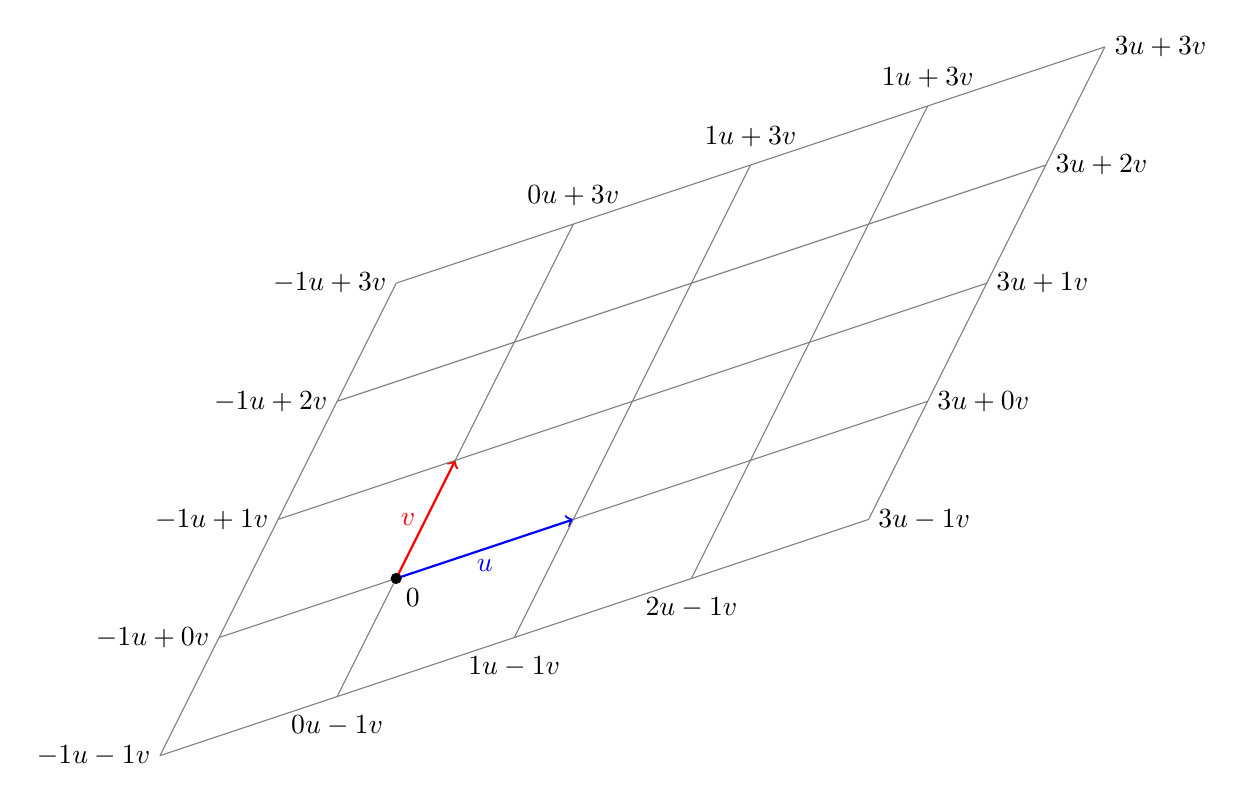
\begin{tikzpicture}[scale=1.5]
\draw[->, thick, blue] (0,0) -- node[below]{$\vect{u}$} (1.5,0.5);
\draw[->, thick, red] (0,0) -- node[left]{$\vect{v}$} (0.5,1);
\draw[-, gray] (-2,-1.5)--(4,0.5);
\draw[-, gray] (-1.5,-0.5)--(0,0);
\draw[-, gray] (1.5,0.5)--(4.5,1.5);
\draw[-, gray] (-1,0.5)--(5,2.5);
\draw[-, gray] (-0.5,1.5)--(5.5,3.5);
\draw[-, gray] (0,2.5)--(6,4.5);
\draw[-, gray] (-2,-1.5)--(0,2.5);
\draw[-, gray] (-0.5,-1)--(0,0);
\draw[-, gray] (0.5,1)--(1.5,3);
\draw[-, gray] (1,-0.5)--(3,3.5);
\draw[-, gray] (2.5,0)--(4.5,4);
\draw[-, gray] (4,0.5)--(6,4.5);
\draw (-2.0,-1.5) node[left]{$-1\vect{u}-1\vect{v}$};
\draw (-1.5,-0.5) node[left]{$-1\vect{u}+0\vect{v}$};
\draw (-1.0,0.5) node[left]{$-1\vect{u}+1\vect{v}$};
\draw (-0.5,1.5) node[left]{$-1\vect{u}+2\vect{v}$};
\draw (0.0,2.5) node[left]{$-1\vect{u}+3\vect{v}$};
\draw (1.5,3.0) node[above=0.75ex]{$0\vect{u}+3\vect{v}$};
\draw (3.0,3.5) node[above=0.75ex]{$1\vect{u}+3\vect{v}$};
\draw (4.5,4.0) node[above=0.75ex]{$1\vect{u}+3\vect{v}$};
\draw (6.0,4.5) node[right]{$3\vect{u}+3\vect{v}$};
\draw (5.5,3.5) node[right]{$3\vect{u}+2\vect{v}$};
\draw (5.0,2.5) node[right]{$3\vect{u}+1\vect{v}$};
\draw (4.5,1.5) node[right]{$3\vect{u}+0\vect{v}$};
\draw (4.0,0.5) node[right]{$3\vect{u}-1\vect{v}$};
\draw (2.5,0.0) node[below=0.75ex]{$2\vect{u}-1\vect{v}$};
\draw (1.0,-0.5) node[below=0.75ex]{$1\vect{u}-1\vect{v}$};
\draw (-0.5,-1.0) node[below=0.75ex]{$0\vect{u}-1\vect{v}$};
\draw[fill] (0,0) circle [radius=1.2pt] node[below right]{$\vect{0}$};
\end{tikzpicture}
\end{center}
As the picture shows, the linear combinations of $\vect{u}$ and
$\vect{v}$ form a 2-dimensional plane through the origin. We say that
this plane is \textbf{spanned}\index{span}\index{vector!span} by the
vectors $\vect{u}$ and $\vect{v}$.  This concept generalizes to more
than two vectors. For example, three vectors may span a 3-dimensional
space (although sometimes, they span only a 2-dimensional space, or
even a line). This motivates the following definition.

\begin{definition}{Span of a set of vectors}{span}
  The set of all linear combinations of the vectors
  $\vect{u}_1, \cdots ,\vect{u}_k$ in $\R^{n}$ is known as the
  \textbf{span}\index{span}\index{vector!span} of these vectors and is written
  as $\sspan\set{\vect{u}_1,\cdots,\vect{u}_k}$. In set notation,
  \begin{equation*}
    \sspan\set{\vect{u}_1,\cdots,\vect{u}_k}
    ~=~ \set{a_1\vect{u}_1+\ldots+a_k\vect{u}_k \mid a_1,\ldots,a_k\in\R}.
  \end{equation*}
\end{definition}

\begin{example}{Vectors in a span}{vector-in-span}
  Let $\vect{u}=\begin{mymatrix}{r} 1 \\ 1 \\ 1 \end{mymatrix}$ and
  $\vect{v}=\begin{mymatrix}{r} 3 \\ 2 \\ 1 \end{mymatrix}^T$. Which
  of the following vectors are elements of
  $\sspan\set{\vect{u},\vect{v}}$?
  \begin{equation*}
    (a)\quad\vect{w} = \begin{mymatrix}{r} 2 \\ 3 \\ 4 \end{mymatrix},
    \qquad
    (b)\quad\vect{z} = \begin{mymatrix}{r} 1 \\ 1 \\ 2 \end{mymatrix}.
  \end{equation*}
\end{example}

\begin{solution}
  (a) For a vector to be in $\sspan\set{\vect{u},\vect{v}}$, it must
  be a linear combination of $\vect{u}$ and $\vect{v}$. Therefore,
  $\vect{w}\in\sspan\set{\vect{u},\vect{v}}$ if and only if we can
  find find scalars $a,b$ such that
  $a\,\vect{u} + b\,\vect{v} = \vect{w}$. We must therefore solve the
  equation
  \begin{equation*}
    a \begin{mymatrix}{r} 1 \\ 1 \\ 1 \end{mymatrix}
    + b \begin{mymatrix}{r} 3 \\ 2 \\ 1 \end{mymatrix}
    = \begin{mymatrix}{r} 2 \\ 3 \\ 4 \end{mymatrix}.
  \end{equation*}
  We write this as an augmented matrix and solve. 
  \begin{equation*}
    \begin{mymatrix}{rr|r}
      1 & 3 & 2 \\
      1 & 2 & 3 \\
      1 & 1 & 4 \\
    \end{mymatrix}
    \sim\ldots\sim
    \begin{mymatrix}{rr|r}
      1 & 0 & 5 \\
      0 & 1 & -1 \\
      0 & 0 & 0 \\
    \end{mymatrix}.
  \end{equation*}
  The solution is $a=5$ and $b=-1$. This means that
  $\vect{w} = 5\vect{u} + (-1)\vect{v}$. Therefore, $\vect{w}$ is an
  element of $\sspan\set{\vect{u},\vect{v}}$.

  (b) We repeat the same method with the vector $\vect{z}$. This time,
  we have to find $a,b$ such that
  $a\,\vect{u} + b\,\vect{v} = \vect{z}$. The system of equations is
  \begin{equation*}
    \begin{mymatrix}{rr|r}
      1 & 3 & 1 \\
      1 & 2 & 1 \\
      1 & 1 & 2 \\
    \end{mymatrix}
    \sim\ldots\sim
    \begin{mymatrix}{rr|r}
      1 & 1 & 2 \\
      0 & 1 & -1 \\
      0 & 0 & 1 \\
    \end{mymatrix},
  \end{equation*}
  which is inconsistent. Therefore, there is no solution. We conclude
  that $\vect{z}$ is not an element of
  $\sspan\set{\vect{u},\vect{v}}$.
\end{solution}

% ----------------------------------------------------------------------
\subsection{CONTINUE HERE} % ###

Consider the following example.

\begin{example}{Span of vectors}{span-vectors}
  Describe the span of the vectors $\vect{u}=\begin{mymatrix}{rrr}
    1  & 1 & 0
  \end{mymatrix}^T$ and
  $\vect{v}=\begin{mymatrix}{rrr}
    3  & 2 & 0
  \end{mymatrix}^T \in \R^{3}$.
\end{example}

\begin{solution}
  You can see that any linear combination of the vectors $\vect{u}$
  and $\vect{v}$ yields a vector of the form
  $\begin{mymatrix}{rrr} x & y & 0
  \end{mymatrix}^T$ in the $XY$-plane. 

  Moreover every vector in the $XY$-plane is in fact such a linear
  combination of the vectors $\vect{u}$ and $\vect{v}$. That's because
  \begin{equation*} \begin{mymatrix}{r}
      x \\
      y \\
      0
    \end{mymatrix} 
    =
    (-2x+3y) \begin{mymatrix}{r}
      1  \\
      1 \\
      0
    \end{mymatrix}
    +
    (x-y)\begin{mymatrix}{r}
      3 \\
      2 \\
      0
    \end{mymatrix} 
  \end{equation*}

  Thus  $\sspan\set{\vect{u},\vect{v}}$ is precisely the $XY$-plane.
\end{solution}

You can convince yourself that no single vector can span the
$XY$-plane. In fact, take a moment to consider what is meant by the
span of a single vector.

However you can make the set larger if you wish. For example consider
the larger set of vectors $\set{\vect{u}, \vect{v},
\vect{w}}$ where $ \vect{w}=\begin{mymatrix}{rrr}
  4 & 5 & 0
\end{mymatrix}^T$. 
Since
the first two vectors already span the entire $XY$-plane, the span is
once again precisely the $XY$-plane and nothing has been gained. Of
course if you add a new vector such as
$ \vect{w}=\begin{mymatrix}{rrr}
  0 & 0 & 1
\end{mymatrix}^T$ then it does span a different space. What is the
span of $\vect{u}, \vect{v}, \vect{w}$ in this case?

The distinction between the sets $\set{\vect{u}, \vect{v}}$ and
$\set{ \vect{u}, \vect{v}, \vect{w}}$ will be made using the concept of
linear independence.

Consider the vectors $\vect{u}, \vect{v}$, and $\vect{w}$ discussed
above. In the next example, we will show how to formally demonstrate
that $\vect{w}$ is in the span of $\vect{u}$ and $\vect{v}$.

